\documentclass{beamer}
\usepackage{graphicx}
\usepackage{amssymb,amsfonts,amsmath}
% color
\usepackage{xcolor}
% \usepackage{tikz,tkz-euclide}
% \usepackage{subfigure}
% \usepackage{parskip}
% \usetikzlibrary{arrows.meta}
% \usetikzlibrary{calc,patterns}
\usefonttheme[onlymath]{serif}
% \usetheme{Berlin}
\title{Divide and Conquer Co-clustering}
\author{WU Zihan}
\begin{document}
\maketitle
% \begin{frame}
%     \frametitle{Catalogue}
%     \tableofcontents
% \end{frame}

\section{Problem}
\begin{frame}
    \frametitle{Introduction}
    \begin{itemize}
        \item Big matrix co-clustering
        \item Partition and merge co-clusters
    \end{itemize}
\end{frame}

\begin{frame}
    \frametitle{Method}
    \begin{itemize}
        \item Partition the big matrix to small ones
        \item Do co-clustering on small ones and get co-clusters on `atom' matrix
    \end{itemize}
    % include figure output.png
    \begin{figure}[htbp]
        \centering
        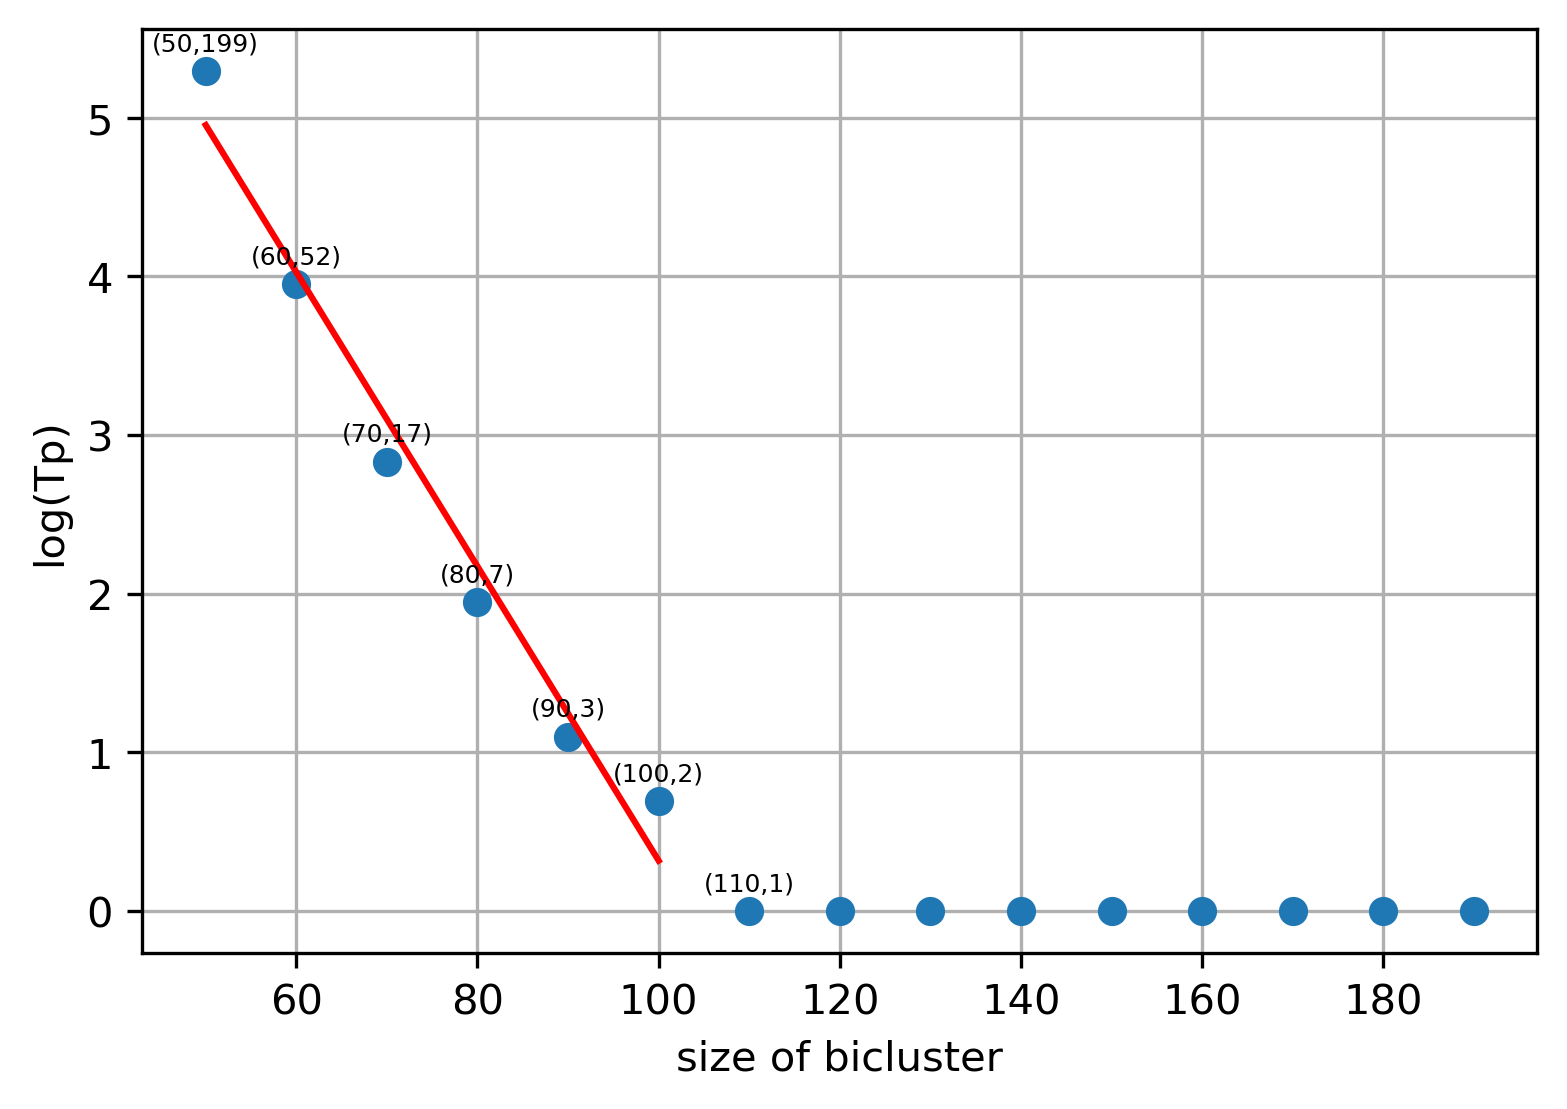
\includegraphics[width=0.5\textwidth]{output.png}
        \caption{Partition and merge}
    \end{figure}
\end{frame}

\begin{frame}
    \frametitle{Simulation}

    \begin{itemize}
        \item $B$ is a $2000\times 2000$ matrix, with $15$ co-clusters. Partitioned to $4\times 4$ sub-matrices.
        \item Several attempts:
              \begin{itemize}
                  \item Merge with intersection conditions:
                        Due to the small size of `atom' co-clusters, the intersection prevents the merge of co-clusters.
                  \item Brute force merge:
                        \begin{itemize}
                            \item $9$ co-clusters are merged from $326$ `atom' co-clusters.
                            \item Acuratelly inside the ground truth.
                            \item \textcolor{red}{But recall is not big enough.}
                        \end{itemize}
                  \item Lower the threshold for `atom' co-clustering:
                        \begin{itemize}
                            \item $143$ co-clusters are merged from $326$ `atom' co-clusters.
                            \item \textcolor{red}{Need to adjust the threshold or find a better way to merge.}
                        \end{itemize}
              \end{itemize}
    \end{itemize}

\end{frame}


\end{document}